%%%%%%%%%%%%%%%%%%%%%%%%%%%%%%%%%%%%%%%%%
% University/School Laboratory Report
% LaTeX Template
% Version 3.1 (25/3/14)
%
% This template has been downloaded from:
% http://www.LaTeXTemplates.com
%
% Original author:
% Linux and Unix Users Group at Virginia Tech Wiki 
% (https://vtluug.org/wiki/Example_LaTeX_chem_lab_report)
%
% License:
% CC BY-NC-SA 3.0 (http://creativecommons.org/licenses/by-nc-sa/3.0/)
%
%%%%%%%%%%%%%%%%%%%%%%%%%%%%%%%%%%%%%%%%%

%----------------------------------------------------------------------------------------
%	PACKAGES AND DOCUMENT CONFIGURATIONS
%----------------------------------------------------------------------------------------

\documentclass{article}

\usepackage{siunitx} % Provides the \SI{}{} and \si{} command for typesetting SI units
\usepackage{graphicx} % Required for the inclusion of images
\usepackage{amsmath} % Required for some math elements 
\usepackage{enumerate} % Required for the enumerate function
\usepackage[siunitx]{circuitikz} % Required for the drawing of circuit diagrams
\usepackage{caption}
\usepackage{graphicx}
\usepackage{subcaption}
\usepackage{xfrac}
\usepackage{float}
\usepackage{enumitem}
\usepackage{pgfplots}
\usepackage{booktabs}
\usepackage{geometry}
\geometry{
	a4paper,
	total={170mm,257mm},
	left=20mm,
	top=20mm,
}

\setlength\parindent{0pt} % Removes all indentation from paragraphs

\renewcommand{\labelenumi}{\alph{enumi}.} % Make numbering in the enumerate environment by letter rather than number (e.g. section 6)

%\usepackage{times} % Uncomment to use the Times New Roman font

\graphicspath{{./fig/}}

%----------------------------------------------------------------------------------------
%	DOCUMENT INFORMATION
%----------------------------------------------------------------------------------------

\title{Analogue Devices \\ Project} % Title

\author{Shane \textsc{Reynolds}} % Author name

\date{\today} % Date for the report

\begin{document}

\maketitle % Insert the title, author and date

\begin{center}
\begin{tabular}{l r}
Date Performed: & May 31, 2017 \\ % Date the experiment was performed
Instructor: & Dr Sina Vafi % Instructor/supervisor
\end{tabular}
\end{center}

% If you wish to include an abstract, uncomment the lines below
% \begin{abstract}
% Abstract text
% \end{abstract}

%----------------------------------------------------------------------------------------
%	SECTION 1
%----------------------------------------------------------------------------------------

\section{Objective}
This project requires the design of a simple current mirror, such that the current which passes through the resistor, $R$, is 150$\si{\micro\ampere}$, and the minimum voltage, $v_{DS}$, is 0.25$\si{\volt}$. The designed circuit is simulated using PSPICE to verify the correct operating characteristics.


%----------------------------------------------------------------------------------------
%	SECTION 2
%----------------------------------------------------------------------------------------

\section{Design}
The circuit topology can be seen in Figure 1. The given device characteristics are $\mu_n C_{ox} = 40 \si{\micro\ampere}$, $V_t = 2 \si{\volt}$, and $\lambda = 0$. The design problem requires that we specify $R$. Additionally the parameters $W$ and $L$ for each of the transistors need to be determined. It is noted that since there is a resistor present in the device, size is not a critical factor when selecting transistors. At this scale micro electro-mechanical (MEM) resistors would be employed to satisfy the resistor requirement. These MEM resistors are orders of magnitude larger than the areas of the transistor devices. The implication is that low cost, larger, transistors can be used without violation of design parameters.\\

Further design considerations surround the decision to use identical transistors for $M_1$, $M_2$, and $M_3$. Selecting transistors with different footprint sizes can make the layout of the device cumbersome, and the final device awkward to implement when dealing with integrated circuits. In this instance, however, we have assumed that this device will not be part of an integrated circuit due to the physical resistor. Hence, it will be assumed that transistors will be matched for simplicities sake. Given this assumption, it is a relatively straight forward task to determine $v_{GS1}$ and $v_{GS2}$. We note that $v_{GS1} = v_{GS2} = 10\si{\volt}$, as shown in the hand calculations. Noting that $v_{G2} = v_{G3}$ and $v_{S2} = v_{S3}$, we see that $v_{GS3} = 10\si{\volt}$ also.

\begin{figure}[H]
	\centering
	\scalebox{1.5}{
	\begin{circuitikz}
		\ctikzset{tripoles/mos style/arrows}
		\ctikzset{bipoles/length=0.75cm}
		\draw
		(0,0) node[nmos] (nmos3) {}
		(nmos3.G) node[nmos,xscale=-1,anchor=G] (nmos2) {}
		(nmos2.D) node[nmos,xscale=-1,anchor=S] (nmos1) {}
		(nmos3.S) -- (nmos2.S)
		(nmos1.G) |- (nmos1.D)
		(nmos3.D) to [R] ($(nmos3.D)+(0,2)$)
		(nmos1.D) |- ($(nmos3.D)+(0,2)$)
		(nmos2.G) |- (nmos2.D)
		(nmos1.B) node[anchor=east] {\tiny $M_1$}
		(nmos2.B) node[anchor=east] {\tiny $M_2$}
		(nmos3.B) node[anchor=west] {\tiny $M_3$}
		(nmos2.S) node[anchor=east,xshift=37,yshift=-5.5] (volt1) {\tiny $-10\si{\volt}$}
		(nmos1.D) node[anchor=north,xshift=28,yshift=25] (volt2) {\tiny$10\si{\volt}$}
		;
	\end{circuitikz}
	}
\caption{The circuit topology of the basic current mirror - the current $I_0$ flows through the resistor in the right hand branch of the circuit.}
\end{figure}

This allows the calculation of the aspect ratio, $\sfrac{W}{L}$, which was found to be 0.11718. This means that we can select some width of the transistor channels, $W$, and calculate the corresponding channel length, $L$. Finally, to get some insight on what resistor value we should implement we can determine an upper bound on acceptable transistor values. Analysis yields that:
\begin{align*}
	R \leq 131.66 \si{\kilo\ohm}
\end{align*}

This upper bound is a theoretical limit for which the transistor voltage $v_{DS3}$ will remain above the 0.25$\si{\volt}$ level - a specification of the design problem. Satisfying this upper bound, however, does not guarantee the transistor will remain in saturation. The upper bound for saturation for the transistor was found to be:
\begin{align*}
	R \leq 80 \si{\kilo\ohm}
\end{align*}  

The channel length, $L$, was chosen arbitrarily to align with the commonly occurring value of 5$\si{\micro\meter}$. The corresponding value for the channel width, $W$, was calculated to be 0.5859$\si{\micro\meter}$. Finally the value for the resistor was chosen to be at the edge of saturation at 80$\si{\kilo\ohm}$.

%----------------------------------------------------------------------------------------
%	SECTION 3
%----------------------------------------------------------------------------------------

\section{Simulation}
The circuit topology was implemented in OrCAD, using the values for the design parameters outlined above. The simulated circuit can be seen in Figure 2.

\begin{figure}[H]
	\centering
	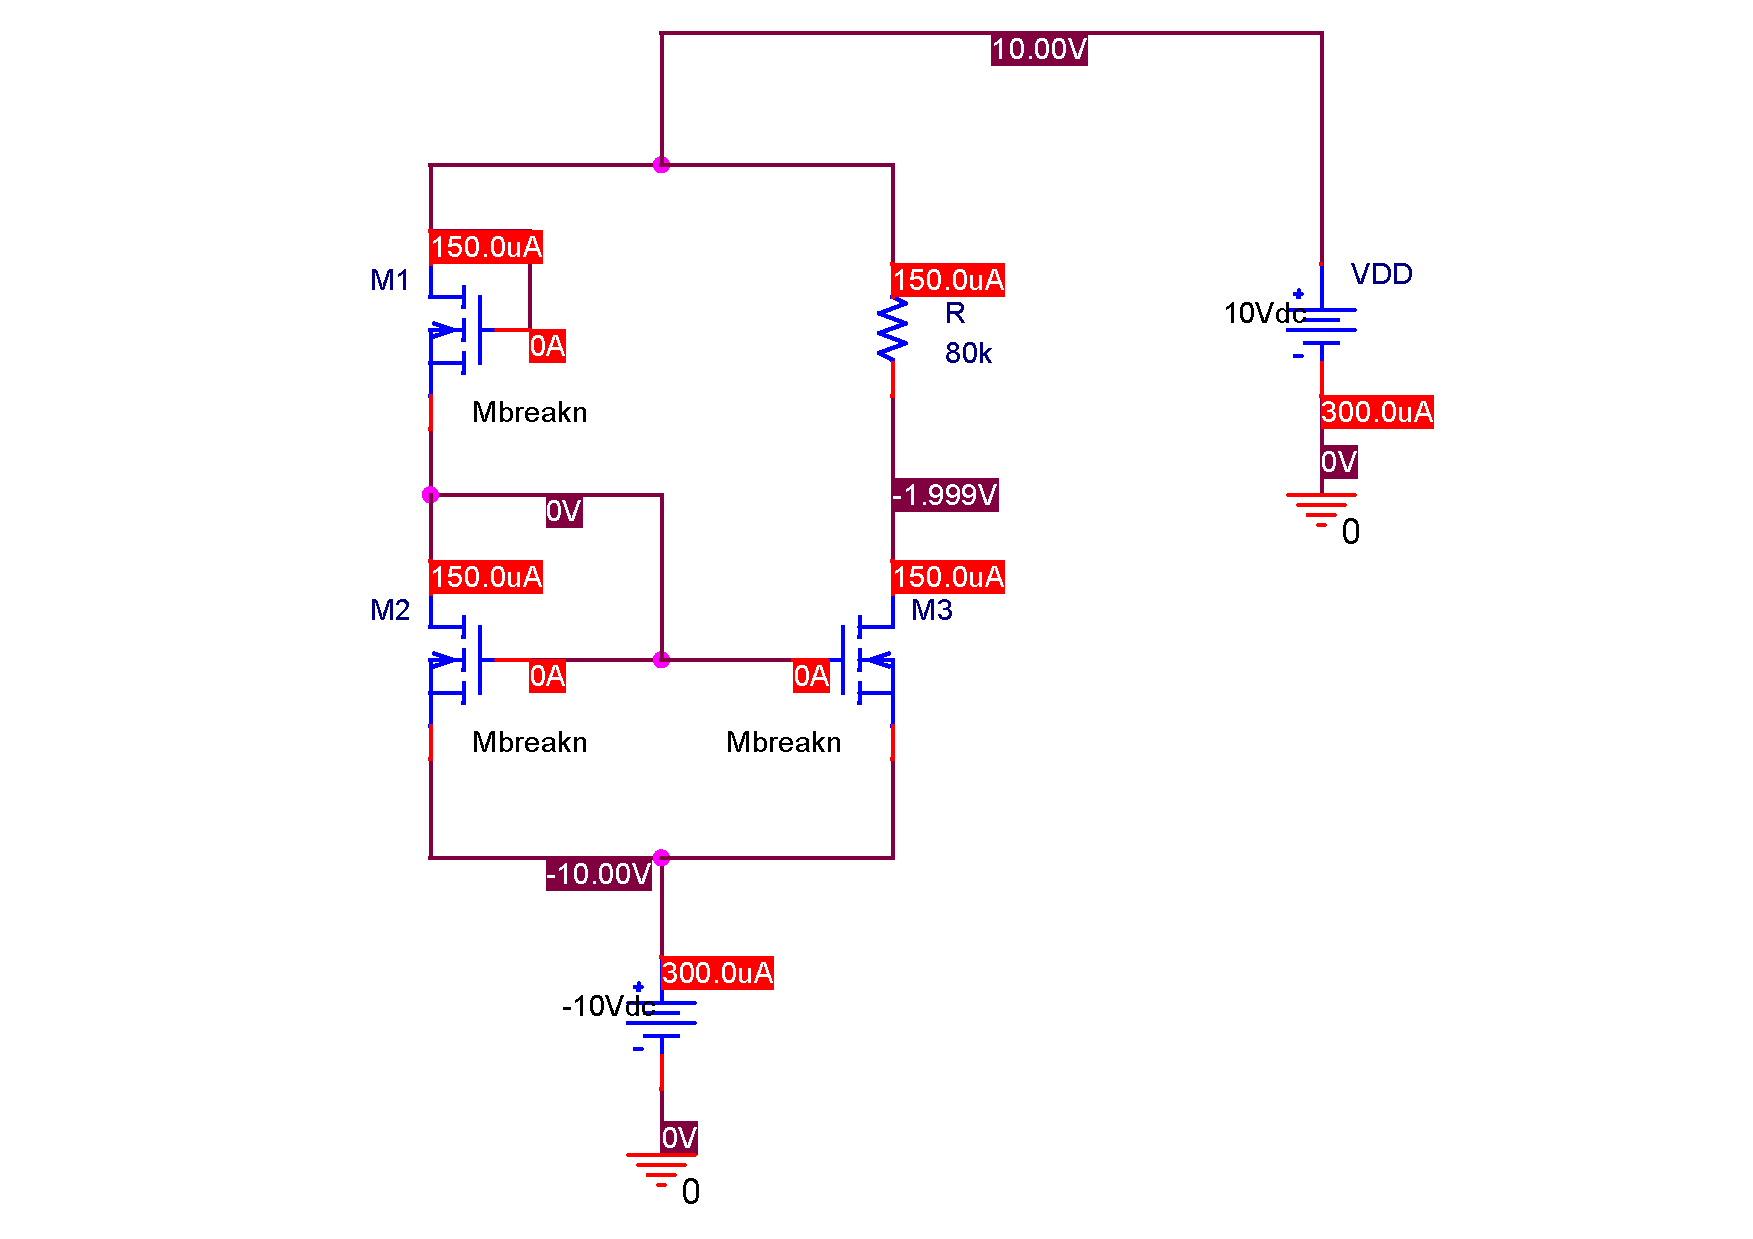
\includegraphics[scale=0.45]{output.pdf}
	\caption{Simulated circuit using design parameters outlined above. The simulation was run in PSPICE.}
\end{figure}


%----------------------------------------------------------------------------------------
%	SECTION 3
%----------------------------------------------------------------------------------------

\section{Discussion}
The values for the current $I_0$ are identical to the design specifications at 150$\si{\micro\ampere}$. Further, we note that transistor 1, 2 and 3 all have $v_{DS}$ values which are greater than the minimum specified value for the design. One aspect of the design worth mentioning is that selecting the resistor at 80$\si{\kilo\ohm}$ leaves the device, $M3$, operating precariously close to the edge of saturation. Choosing a resistor value lower than 80$\si{\kilo\ohm}$ would see an increase in the stability of the circuit performance. Power consumption for the device will not change given that there is a fixed current through both branches of the circuit, over a fixed potential difference of 20$\si{\volt}$.

\section{Conclusion}
The design criteria were met with no exceptions, and the device performed in simulation as expected.


\end{document}